\documentclass{beamer}
\usetheme{metropolis}         
\title{Deep Checker}

\subtitle{Apprentissage statistique et intelligence artificielle}
\date{}
\author{Arthur Correnson, Igor Martayan, Manon Sourisseau}
\titlegraphic{\hfill
\includegraphics[height=1.5cm]{im/logo.pdf}}
\institute{Projet de Statistiques, ENS, 2021}
\begin{document}

{\metroset{background=dark}\maketitle}

  \begin{frame}{Introduction}
    \begin{columns}
        \column{0.6\textwidth}
        \begin{itemize}
            \item Construction d'une \alert{heuristique} évaluant la qualitée des coups
            \item Nécéssité d'un grand nombre de partie de jeu de dames
        \end{itemize}
        \column{0.4\textwidth}
        \begin{figure}
            \centering
            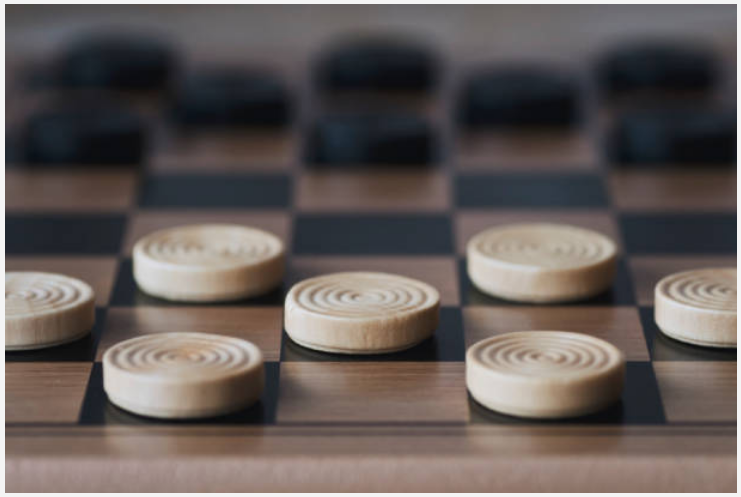
\includegraphics[width=\columnwidth]{im/dames.png}
        \end{figure}
    \end{columns}
  \end{frame}

  \begin{frame}{Plan de la présentation}
    \setbeamertemplate{section in toc}[sections numbered]
    \tableofcontents
\end{frame}

{\metroset{background=dark}\section{Génération de données et simulateur}}
\begin{frame}{Génération de données}
    \begin{itemize}
        \item Besoin d'un \alert{grand nombre de données}
        \item Générer beaucoup de parties \alert{rapidemment} et de manière \alert{compacte} en mémoire
        \item Ecriture d'un simulateur dans le langage \alert{C}
    \end{itemize}
\end{frame}

\begin{frame}{Création d'un simulateur}
    \begin{columns}
        \column{0.6\textwidth}
        \begin{itemize}
            \item 64 cases, 32 cases possibles 
            \item 3 états possibles par cases :\newline
             Vide, pion blanc, pion noir
        \end{itemize}
        Représentation de l'état du plateau par un entier de 64 bits (\alert{2 x 32 bits})
        exemple : 1111 1111 1111 0000 0000 0000 0000 0000 //   0000 0000 0000 0000 0000 1111 1111 1111

        \column{0.4\textwidth}
        \begin{figure}
            \centering
            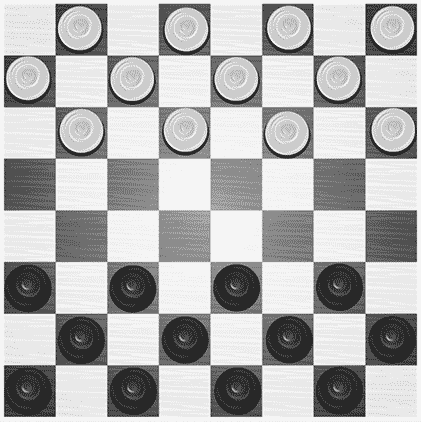
\includegraphics[width=\columnwidth]{im/dames2.png}
        \end{figure}
    \end{columns}
\end{frame}
\begin{frame}{Données et performances}
    \begin{itemize}
        \item Les données sont stockées dans un fichier texte. \newline
        (perte d'éfficacité contre simplicité de traitement des données)
        \item Performances très satisfaisantes :\newline
        \alert{10 000} parties générées en environ \alert{1 secondes}, sur un ordinateur ordinaire.
    \end{itemize}
\end{frame}
{\metroset{background=dark}\section{Modèles et heuristiques}}
\begin{frame}{Modèles et heuristiques}
    On souhaite construire une heuristique qui attribut un \alert{score} à un coup donné, selon la \alert{qualité} du coup. 
    Plusieurs approches pour déterminer l'heuristique :
    \begin{itemize}
        \item Régression par les K plus proches voisins (KNN)
        \item Réseaux de perceptron
    \end{itemize}
    Le but est de jouer le coup possible ayant le meilleur score.
\end{frame}

\begin{frame}{Modélisation du problème}

    Étant donné un ensemble $\mathcal{X}$de parties simulées. 
    n souhaite donner une première approcximation de l'heuristique $h$.
    
    \begin{itemize}
        \item On associe chaque coup apparaissant dans une partie $P \in X$ un score
        \item Le score final d'un coup $c$ est la moyenne des scores qui lui sont attribués sur l'ensemble des parties dans $X$
    \end{itemize}

\end{frame}

{\metroset{background=dark}\section{Régression aux k plus proches voisins}}

\begin{frame}{Régression par KNN}
    KNN : méthode de régression aux \alert{K plus proche voisins}.
    On définit la distance entre deux coups par la \alert{distance d'édition} :
    $$ \langle c_1, c_2 \rangle_{KNN} = \ \rVert c_1 \oplus c_2 \lVert_1 $$
    $\rightarrow$ Les coups sont représentés comme des entiers de 128 bits. 
    \begin{itemize}
        \item On calcule la distance du coup donné avec tous les autres coups.
        \item Le score attribué au coup donné correspond à \alert{la moyenne des scores} des K plus proches voisins. 
    \end{itemize}

\end{frame}

\begin{frame}{Résultat et performances de KNN}
    \begin{center}
        \begin{tabular}{ | l | c | }
          \hline
          Victoires du joueur 1 (KNN) & Victoires du joueur 2 (Aléatoire)  \\ \hline
          18 & 32  \\ \hline
        \end{tabular}
      \end{center}

Cette version de l'heuristique est peu satisfaisante

\end{frame}

{\metroset{background=dark}\section{Réseau de perceptron}}

\begin{frame} {Nouveau calcul de score}
    \begin{itemize}
        \item Nouvelle fonction d'évaluation : \newline
        $\lVert.\rVert_i : D_i \to \mathbb{N}$ définie comme : $\lVert d \rVert_i = p(d).v(d)$
        \begin{itemize}
            \item $D_i$ : Ensemble des états du damier vu par le joueur 1
            \item $p(d) \in \mathbb{N}$ : Nombre de pions mangé depuis l'état $d$
            \item  $v(d) = 1$ si le joueur 1 gagne, $v(d) = 0$ sinon
        \end{itemize}
        \item On construit maintenant une fonction $w_i(c)$ telle que $w_i(d) = \lVert c \lVert_i$ si $d \in D_i$ et $w_i(d) = 0$ sinon
        \item Pour chaque état de damier $d$ apparaissant dans l'ensemble des parties de $\mathcal{DB}$, $h(d) = \frac{1}{N}\Sigma w_i(d)$ avec $N$ le nombre de parties $P_i$ tels que $w_i(d) \neq 0$ ($d$ est l'un des états pris par le damier dans $P_i$)
         
    \end{itemize}
\end{frame}

\begin{frame} {Réseau de neurones type perceptron multicouche}
    \begin{itemize}
        \item Entrées : vecteurs de 64 bits (représentant un unique damier)
        \item Coeur du réseau : 4 couches intermédiaires
        \item Noeuds du réseau : fonction d'activation \alert{relu}
        \item Sortie du réseau de dimension 1 (régression) : combinaison linéraire des 16 sorties de la dernière couche puis d'une application de \alert{relu}
    \end{itemize}
\end{frame}

\begin{frame} {Résultats du réseau perceptron}
    \begin{center}
        \begin{tabular}{ | l | c | }
          \hline
          Victoires du joueur 1 (MLP) & Victoires du joueur 2 (Aléatoire)  \\ \hline
          50 & 0  \\ \hline
        \end{tabular}
      \end{center}

$\rightarrow$ Heuristique bien plus satisfaisantes
\end{frame}

\end{document}